
%%%%%%%%%%%%%%%%%%%%%%% file typeinst.tex %%%%%%%%%%%%%%%%%%%%%%%%%
%
% This is the LaTeX source for the instructions to authors using
% the LaTeX document class 'llncs.cls' for contributions to
% the Lecture Notes in Computer Sciences series.
% http://www.springer.com/lncs       Springer Heidelberg 2006/05/04
%
% It may be used as a template for your own input - copy it
% to a new file with a new name and use it as the basis
% for your article.
%
% NB: the document class 'llncs' has its own and detailed documentation, see
% ftp://ftp.springer.de/data/pubftp/pub/tex/latex/llncs/latex2e/llncsdoc.pdf
%
%%%%%%%%%%%%%%%%%%%%%%%%%%%%%%%%%%%%%%%%%%%%%%%%%%%%%%%%%%%%%%%%%%%


\documentclass[runningheads,a4paper]{llncs}

\usepackage{amssymb,amsmath}
\setcounter{tocdepth}{3}
\usepackage{graphicx}
\usepackage{url}
\usepackage{color,subfig}

%Definitions
\urldef{\mailsa}\path|{maruthi_narayanan,benjamin_kimia}@brown.edu|
\def\eg{\emph{e.g.}}
\def\FigureFont{\small}
\def\ie{\emph{i.e.}}
\def\etc{\emph{etc. }}
\newcommand{\etal}{{\it et al. }}


\begin{document}

\mainmatter  % start of an individual contribution

% first the title is needed
\title{Supplemental Material: Bottom-Up Perceptual Organization of Images into Object Part Hypotheses}

% a short form should be given in case it is too long for the running head
\titlerunning{Bottom-Up Perceptual Organization of Images into Object Part Hypotheses}

% name author
\author{Maruthi Narayanan \and Benjamin Kimia}
%
\authorrunning{Maruthi Narayanan and Benjamin Kimia}


\institute{Brown University\\
School of Engineering\\
Providence, RI 02912\\
\mailsa\\
\url{http://vision.lems.brown.edu}}

\maketitle

In what follows we provide supplementary data which was too detailed to include in the paper in the given page limit. Section 1 discusses the computational aspects of our pipeline. In Section 2 more details about the experimental procedure for evaluating fragmentation along with more examples of fragmentation versus segmentation are presented. Section 3 discusses how transforms are identified. Section 4 discusses the likelihood associated with each transform.


\section{Computational Details} In all experiments, each image was processed across multiple scales. Edges were extracted using the globalPb ({\it gPb}) algorithm~\cite{Maire:etal:CVPR08}. To recover the proper orientation of {\it gPb} edgels, a third-order correction was applied and grouped~\cite{Tamrakar:Kimia:ICCV07}. The shock graph was computed across scales with these contour maps. The root level of the {\em containment graph} was initialized with a subset of medial fragments having a high contour ratio, real vs imaginary contours, greater than 0.4. The path threshold on node expansion was set to 0.1 confidence. Medial fragments were extracted out of the containment graph if the contour ratio was greater than 0.4 and the cumulative probability of the node was greater than the path threshold. 

\section{Fragmentation versus Segmentation}
To evaluate fragmentation versus segmentation experiments were based on the database used in~\cite{Endres:Hoiem:ECCV10}, which are annotations of images from the BSDS300 Test set. This dataset can be  found at \url{http://vision.cs.uiuc.edu/proposals}.  For each ground truth object, the {\it percent-object recall}, is examined as a function of the number of fragments, both for our method and for segments from~\cite{Carreira:Sminchisescu:PAMI12} which we obtained from the code kindly shared by them: \url{http://sminchisescu.ins.uni-bonn.de/code/cpmc}. Additional examples are shown in Table~\ref{table:example_frag_measure}.


% \begin{figure}[h!]
%  %\hspace{-0.9cm}
%   \centering
%   \begin{tabular}[!ht]{cc}
%     a)\includegraphics[width=0.48\linewidth]{figs/108070_best_fragments.jpg} &
%     b)\includegraphics[width=0.48\linewidth]{figs/pami_cpmc/108070_best_fragments.jpg} \\
%     c)\includegraphics[width=0.48\linewidth]{figs/Cpmc_vs_our_method_108070.pdf} &
%     d) 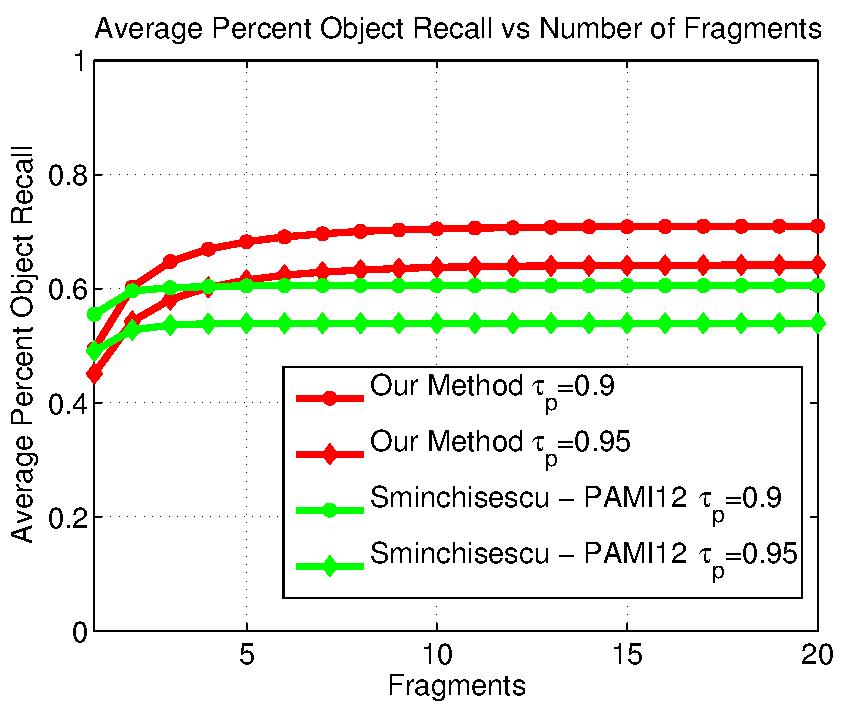
\includegraphics[width=0.48\linewidth]{figs/03_12_12_fragmentation_score_full_bsdtest.pdf}  \\
%   \end{tabular}
%   \caption{(a,b) The top performing fragments (Best Jaccard Index) for our method is similar to that of CPMC~\cite{Carreira:Sminchisescu:PAMI12}. However
%     as additional fragments are include the performance of our fragments is
%     distinguished from that of CPMC~\cite{Carreira:Sminchisescu:PAMI12} as
%     shown in (c). (d) Average Fragmentation Measure at $\tau_p=0.90,0.95$ for Test Set of BSDS300. }
%     \label{fig:cpmc_vs_ours1}

% \end{figure}

% \begin{table}[h]
% \caption{Example Image from BSDS300 Test Set comparing Our Method versus CPMC. }
% \centering
% \hspace*{-0.6cm}
%   \begin{tabular}{|c | c | c | c | c | c | c |}
%     \hline
%     Method & {\bf Top 1} & {\bf Top 2 } & {\bf Top 3 } & {\bf Top 4} & {\bf Union - 20} & {\bf Object Recall} \\
%     \hline
%     Our  Method &
%     \includegraphics[width=0.14\linewidth]{figs/108070_top_1_fragments.jpg} &
%     \includegraphics[width=0.14\linewidth]{figs/108070_top_2_fragments.jpg} &
%     \includegraphics[width=0.14\linewidth]{figs/108070_top_3_fragments.jpg} &
%     \includegraphics[width=0.14\linewidth]{figs/108070_top_4_fragments.jpg} &
%     \includegraphics[width=0.14\linewidth]{figs/108070_top_20_fragments_montage.jpg} &
%     \includegraphics[width=0.14\linewidth]{figs/108070_object_recall_vs_fragments.pdf}\\
%     \hline
%     CPMC~\cite{Carreira:Sminchisescu:PAMI12} &
%     \includegraphics[width=0.14\linewidth]{figs/pami_cpmc/108070_top_1_fragments.jpg} &
%     \includegraphics[width=0.14\linewidth]{figs/pami_cpmc/108070_top_2_fragments.jpg} &
%     \includegraphics[width=0.14\linewidth]{figs/pami_cpmc/108070_top_3_fragments.jpg} &
%     \includegraphics[width=0.14\linewidth]{figs/pami_cpmc/108070_top_4_fragments.jpg} &
%     \includegraphics[width=0.14\linewidth]{figs/pami_cpmc/108070_top_20_fragments_montage.jpg} &
%   \includegraphics[width=0.14\linewidth]{figs/pami_cpmc/108070_object_recall_vs_fragments.pdf} \\
%     \hline
%   \end{tabular}
% \label{table:frag_measure}
% \end{table}



\begin{table}[h!]
\label{fig:example_frag_measure}
\caption{Fragmentation Measure for a sample of BSDS300 Test}
\centering
\hspace*{-0.6cm}
  \begin{tabular}{|c | c | c | c | c | c | c |}
    \hline
    {\bf Top 1 } & {\bf Top 2} & {\bf Top 3 } & {\bf Top 4 } & {\bf Top 5} & {\bf Union - 20} & {\bf Object Recall} \\
    \hline
    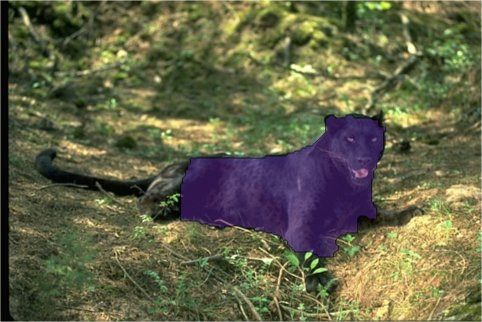
\includegraphics[width=0.14\linewidth]{figs/304034_top_1_fragments.jpg}&
    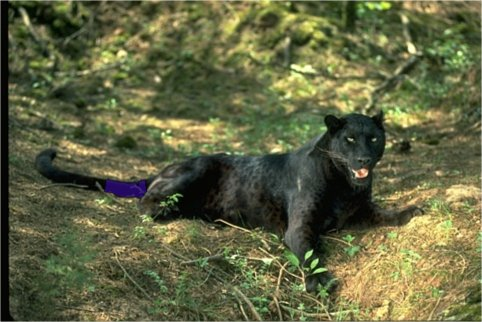
\includegraphics[width=0.14\linewidth]{figs/304034_top_2_fragments.jpg}&
    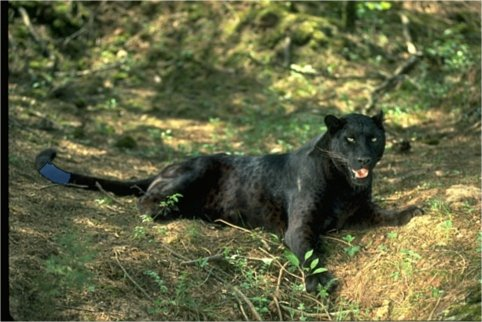
\includegraphics[width=0.14\linewidth]{figs/304034_top_3_fragments.jpg}&
    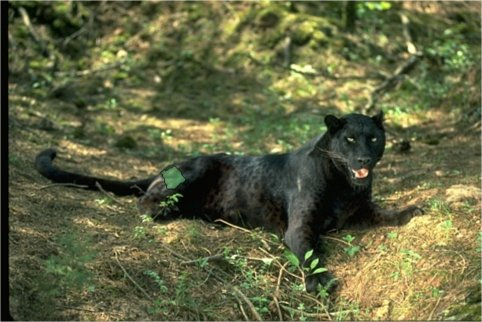
\includegraphics[width=0.14\linewidth]{figs/304034_top_4_fragments.jpg}&
    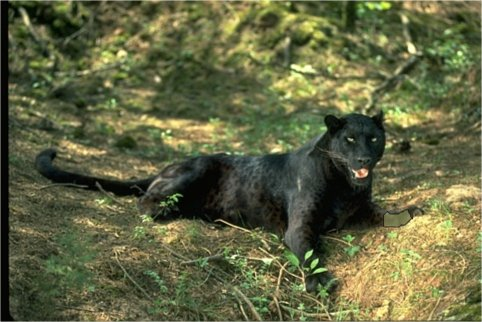
\includegraphics[width=0.14\linewidth]{figs/304034_top_5_fragments.jpg}&
    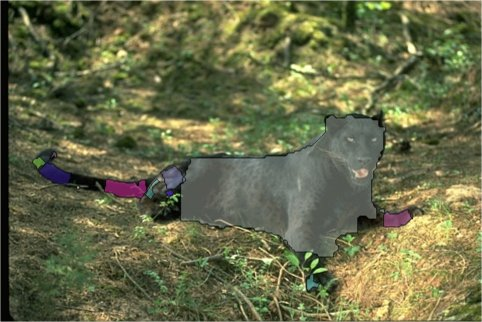
\includegraphics[width=0.14\linewidth]{figs/304034_top_20_fragments_montage.jpg}&
    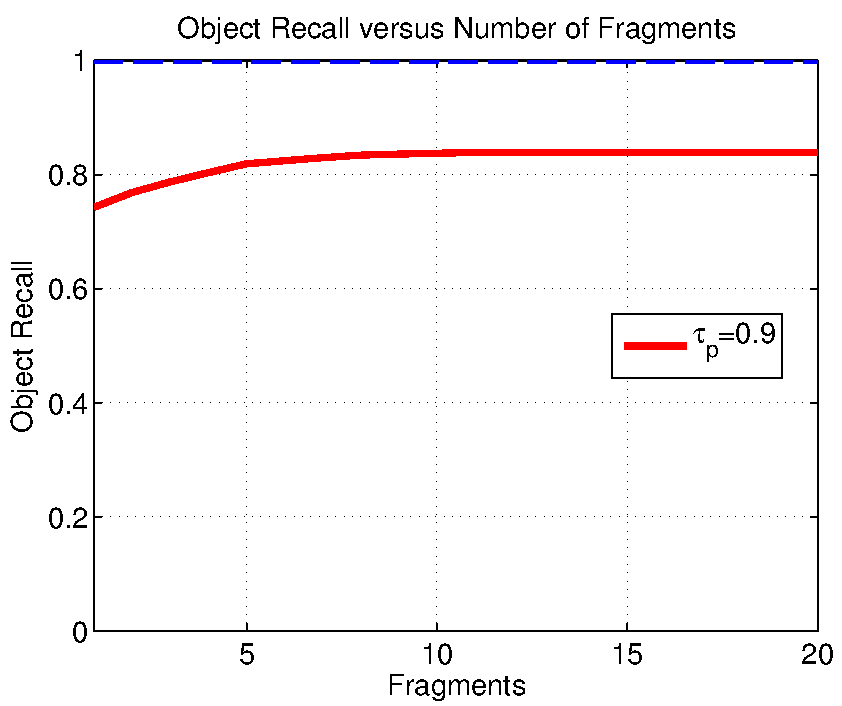
\includegraphics[width=0.14\linewidth]{figs/304034_object_recall_vs_fragments.pdf} \\
    \hline
%     \includegraphics[height=0.15\linewidth]{figs/189080_top_1_fragments.jpg}&
%     \includegraphics[height=0.15\linewidth]{figs/189080_top_2_fragments.jpg}&
%     \includegraphics[height=0.15\linewidth]{figs/189080_top_3_fragments.jpg}&
%     \includegraphics[height=0.15\linewidth]{figs/189080_top_4_fragments.jpg}&
%     \includegraphics[height=0.15\linewidth]{figs/189080_top_5_fragments.jpg}&
%     \includegraphics[height=0.15\linewidth]{figs/189080_top_20_fragments_montage.jpg}&
%    \includegraphics[width=0.14\linewidth]{figs/189080_object_recall_vs_fragments.pdf}\\
%    \hline
    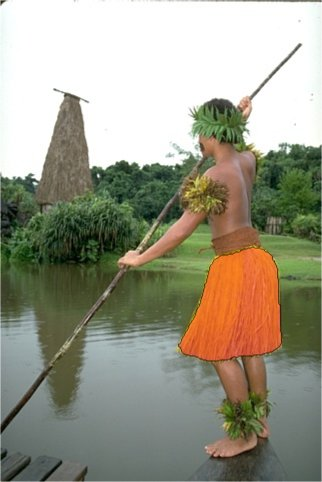
\includegraphics[height=0.15\linewidth]{figs/101087_top_1_fragments.jpg}&
    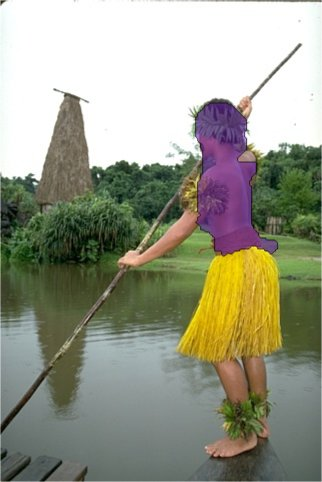
\includegraphics[height=0.15\linewidth]{figs/101087_top_2_fragments.jpg}&
    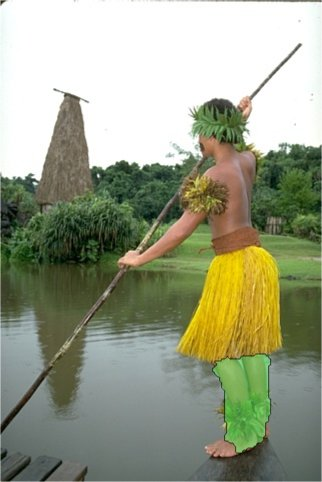
\includegraphics[height=0.15\linewidth]{figs/101087_top_3_fragments.jpg}&
    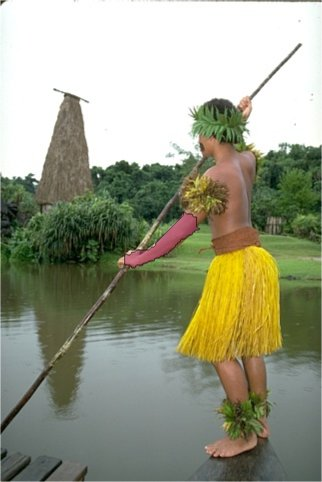
\includegraphics[height=0.15\linewidth]{figs/101087_top_4_fragments.jpg}&
    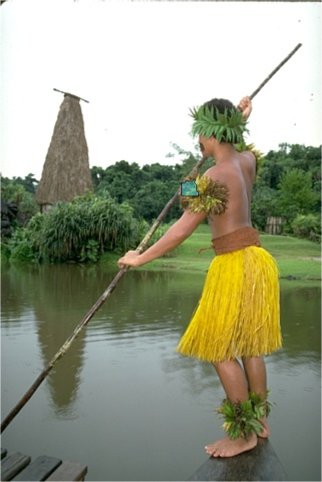
\includegraphics[height=0.15\linewidth]{figs/101087_top_5_fragments.jpg}&
    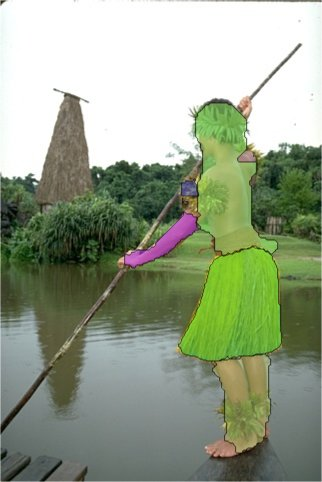
\includegraphics[height=0.15\linewidth]{figs/101087_top_20_fragments_montage.jpg}&
    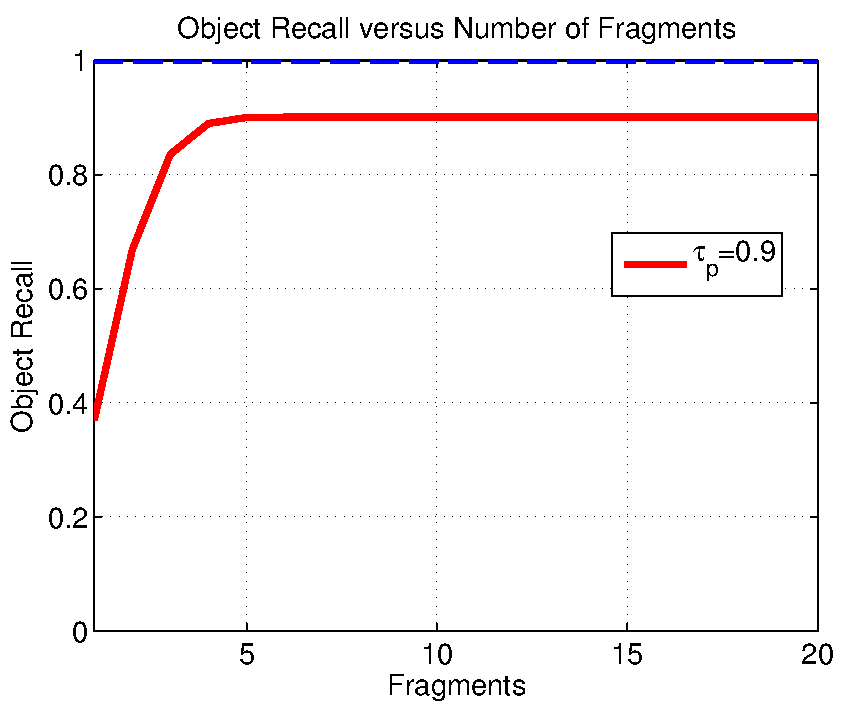
\includegraphics[width=0.14\linewidth]{figs/101087_object_recall_vs_fragments.pdf} \\
    \hline
    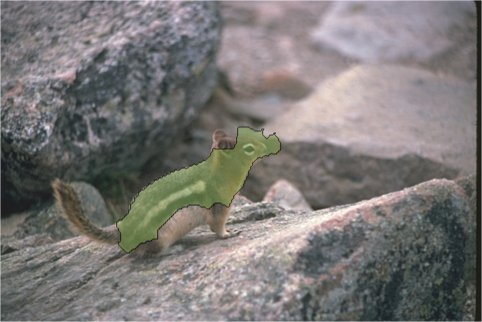
\includegraphics[width=0.14\linewidth]{figs/123074_top_1_fragments.jpg}&
    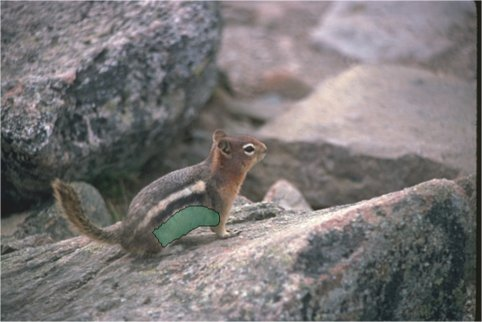
\includegraphics[width=0.14\linewidth]{figs/123074_top_2_fragments.jpg}&
    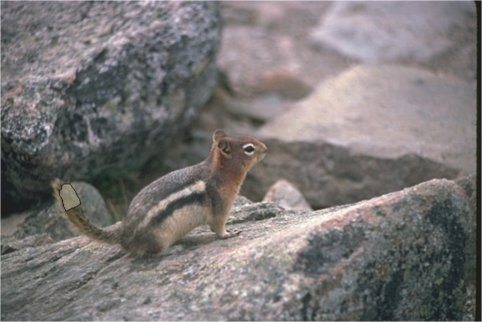
\includegraphics[width=0.14\linewidth]{figs/123074_top_3_fragments.jpg}&
    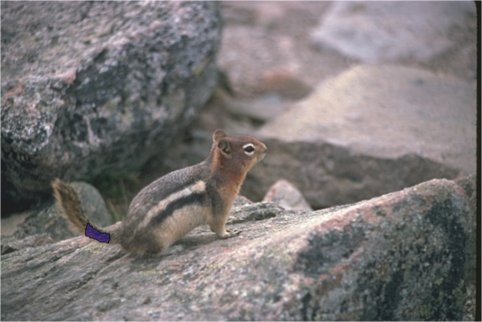
\includegraphics[width=0.14\linewidth]{figs/123074_top_4_fragments.jpg}&
    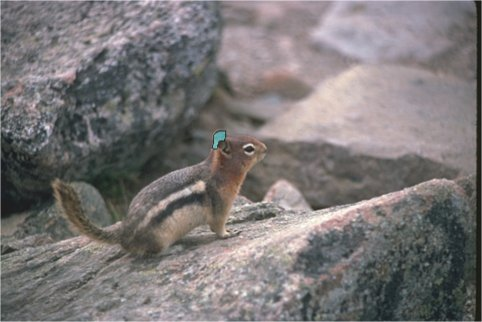
\includegraphics[width=0.14\linewidth]{figs/123074_top_5_fragments.jpg}&
    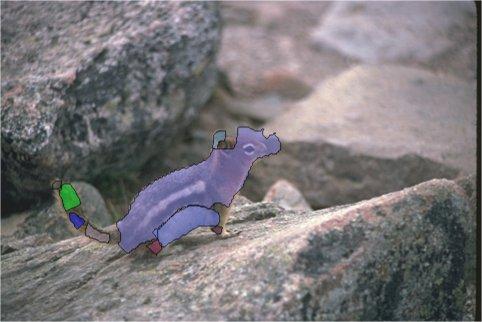
\includegraphics[width=0.14\linewidth]{figs/123074_top_20_fragments_montage.jpg}&
    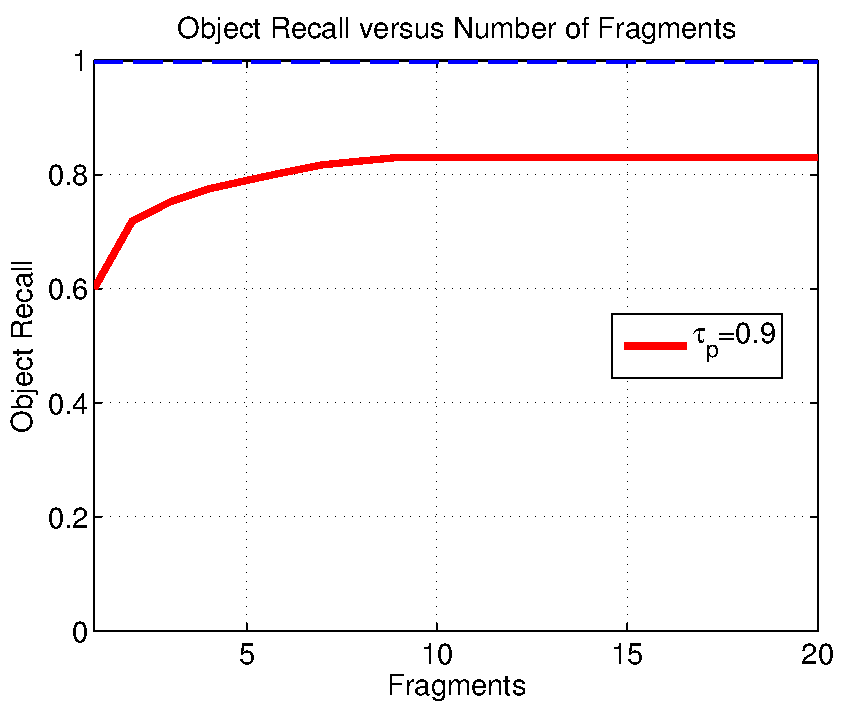
\includegraphics[width=0.14\linewidth]{figs/123074_object_recall_vs_fragments.pdf} \\
    \hline
  \end{tabular}
\label{table:example_frag_measure}
\end{table}
%\includegraphics[width=0.5\linewidth]{figs/108070_object_recall_vs_fragments.pdf}
% \includegraphics[width=0.5\linewidth]{figs/pami_cpmc/108070_object_recall_vs_fragments.pdf}

\section{Identification of Transforms}

A key element in implementing our approach is how to find all possible transforms which a fragment can undergo. The shock graph itself provides a clue to the potential  gap closure ({\em gap transform}) and the potential spurious elements ({\em loop transform}). 

The identification of all types of gap transforms centers around first locating endpoints. A brute force approach would be to consider all pairs of endpoints within the composite graph as possible gap completions. However this is not necessary, as branches of the shock graph are classified by their interacting pair of contour elements (point,line). A {\em degenerate}~\cite{Giblin:Kimia:IJCV03} shock branch is formed by waves emanating from two contour endpoints, where as a {\em semi-degenerate}~\cite{Giblin:Kimia:IJCV03} shock branch is formed by the interaction of an endpoint with a line. {\bf Gap I} in Figure 4 of the submitted paper, is detected by finding {\em degenerate} shock branches, and {\bf Gap 4} is found by locating {\em semi-degenerate} shock branches.See Figure~\ref{fig:gap-edges} for an example of each kind. All the rest of the gap sub-types fall into one of these two categories.

\begin{figure}[h!]
\centerline{
\begin{tabular}{cccccc}
   {\small (a) } & 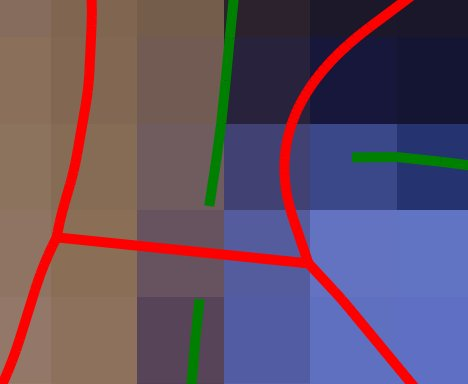
\includegraphics[width=2.5cm]{figs/hidden-edges-closed-gaps-image.jpg} &
   {\small (b) } & 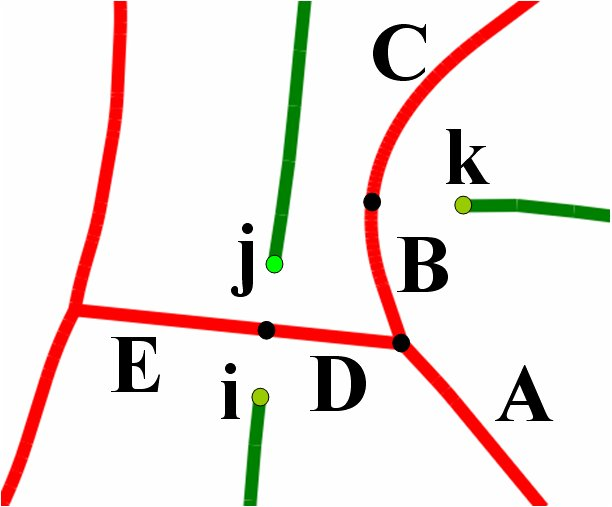
\includegraphics[width=2.5cm]{figs/degenerate-edges.jpg} &
   {\small (c) } & 
\includegraphics[width=2.5cm]{figs/hidden-edges-closed-gaps.jpg}\\
\end{tabular}} 
\vspace{-0.2 cm} \caption{{\small (a) \textcolor{green}{Image curves} shown in green
and \textcolor{red}{shock graph} in red (b) D, E and A are degenerate edges,
suggesting the closure of (i-j), (j-i) and (i-k) respectively. B and
C are semi-degenerate edges suggesting to form a T-junction from k
to the contour. (b) Completion curves in blue after the gap (i-j) is
closed and a T-junction is formed based on the closure criteria.}}
\label{fig:gap-edges} \vspace{-0.4 cm}
\end{figure}

Many contours interfere with the formation of an object fragment. These contours interfere with process of shock formation and cause {\em loops} to form in the shock graph. Transformations of this type can be detected by looking for cycles in the shock graph. Rather than explicitly look for cycles in the graph, we can directly index into loops using contour fragments since each maps to a cycle in shock graph. 




\section{Probability of Transforms}
\label{sec:prob_transform}

The {\it gap completion transform} considers the option of completing a gap by a completion curve, thus joining and merging  two  curve fragments whose endpoints created the gap. Two types of cues can generally help make a determination of completion: shape and appearance. The current algorithm only takes advantage of the shape cue; appearance will be used in future
to discriminate completion better. The shape cue relies on the Gestalt cue of {\em good contour continuation}, as captured by the publicly available
code~\url{http://vision.lems.brown.edu/content/available-software-and-databases} of the Euler Spiral completion~\cite{Kimia:Euler:Spiral:IJCV03}, which is
used to join a pair of curve endpoints. 

The estimation of a gap completion likelihood is based on, supervised learning based on the given completion curve. A training set was constructed out of a random set of ETHZ images,
\url{http://www.vision.ee.ethz.ch/datasets/index.en.html}.
Specifically, gaps were identified and a local window around the gap, together
with the proposed Euler Spiral Completion was presented to subjects, Figure~\ref{fig:training}, who where asked whether they would close the gap with the proposed completion.
This approach is similar to the work by Geisler~\cite{Geisler:vision:journal}. The full training set consists of a user defined label (\textcolor{blue}{yes=1}, \textcolor{red}{no=0}), and each possible gap completion is represented by its Euler Spiral parameters $\{\gamma, \kappa_0,l\}$, where $\gamma$, $\kappa_0$, and $l$ represent derivative of curvature, initial curvature, and arc-length, respectively. To properly account for scale, parameters  $\gamma$ and $\kappa_0$ where scale-normalized  by factors $d^2$ and $d,$ respective, where $d$ represent the distance between the two contour endpoints.

%\vspace{-2cm}

\begin{figure}[h]
  \subfloat[\textcolor{red}{Contours}
  \textcolor{blue}{Completion Curve}, Training example for users to judge]
  {
    \label{fig:training}
    \begin{tabular}[!ht]{|c|c|}
      \hline
      \textcolor{red}{Unlikely Gaps} & \textcolor{blue}{Likely Gaps} \\
      \hline
      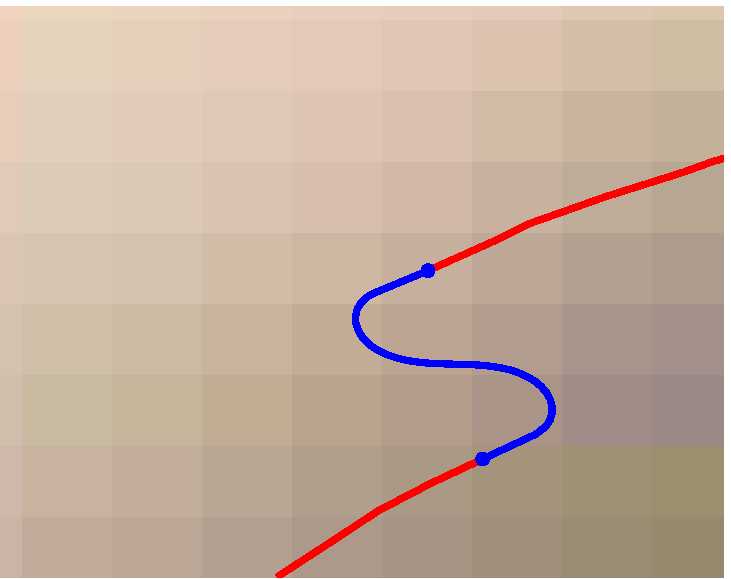
\includegraphics[width=0.25\linewidth]{figs/bad_gap1.pdf} &
      \includegraphics[width=0.25\linewidth]{figs/good_gap1.pdf} \\
      \hline
      \includegraphics[width=0.25\linewidth]{figs/bad_gap2.pdf} &
      \includegraphics[width=0.25\linewidth]{figs/good_gap2.pdf} \\
      \hline
    \end{tabular}
  }
  \begin{tabular}{c}
    \subfloat[Feature space]{
      \label{fig:feature_space}
      \includegraphics[width=0.45\linewidth]{figs/solution_space.pdf}}\\
    \subfloat[Decision Boundary SVM]{
      \label{fig:decision_boundary}\includegraphics[width=0.45\linewidth]{figs/surface_c10_r8_v2.jpg}}\\
  \end{tabular}
  \caption{The steps in training  a gap completion likelihood measure.}
\end{figure}

A decision boundary, Figure~\ref{fig:decision_boundary}, in the feature space $\{\gamma d^2,\kappa_0 d,l\}$, Figure~\ref{fig:feature_space}, was learned using Support Vector Machines (SVM), \url{http://cmp.felk.cvut.cz/cmp/software/stprtool}. To derive the conditional probability, $p(gap|\gamma,\kappa_0,l)$, the SVM scores were converted into probabilities using the method by Platt~\cite{Platt:99}. The probability of removing a contour, {\it loop transform }, is inversely related to the minimum cost of removing a contour which is defined as how likely it participates in a gap. 

\begin{equation}
p(loop\_removal)=1-\min_ip^i(gap\_completion|\gamma,\kappa_0,l)
\label{eq:loop_prob}
\end{equation} 

\bibliographystyle{splncs}


%%%%%%%%%%%%%%%%%%%%%%% file typeinst.tex %%%%%%%%%%%%%%%%%%%%%%%%%
%
% This is the LaTeX source for the instructions to authors using
% the LaTeX document class 'llncs.cls' for contributions to
% the Lecture Notes in Computer Sciences series.
% http://www.springer.com/lncs       Springer Heidelberg 2006/05/04
%
% It may be used as a template for your own input - copy it
% to a new file with a new name and use it as the basis
% for your article.
%
% NB: the document class 'llncs' has its own and detailed documentation, see
% ftp://ftp.springer.de/data/pubftp/pub/tex/latex/llncs/latex2e/llncsdoc.pdf
%
%%%%%%%%%%%%%%%%%%%%%%%%%%%%%%%%%%%%%%%%%%%%%%%%%%%%%%%%%%%%%%%%%%%


\documentclass[runningheads,a4paper]{llncs}

\usepackage{amssymb,amsmath}
\setcounter{tocdepth}{3}
\usepackage{graphicx}
\usepackage{url}
\usepackage{color,subfig}

%Definitions
\urldef{\mailsa}\path|{maruthi_narayanan,benjamin_kimia}@brown.edu|
\def\eg{\emph{e.g.}}
\def\FigureFont{\small}
\def\ie{\emph{i.e.}}
\def\etc{\emph{etc. }}
\newcommand{\etal}{{\it et al. }}


\begin{document}

\mainmatter  % start of an individual contribution

% first the title is needed
\title{Supplemental Material: Bottom-Up Perceptual Organization of Images into Object Part Hypotheses}

% a short form should be given in case it is too long for the running head
\titlerunning{Bottom-Up Perceptual Organization of Images into Object Part Hypotheses}

% name author
\author{Maruthi Narayanan \and Benjamin Kimia}
%
\authorrunning{Maruthi Narayanan and Benjamin Kimia}


\institute{Brown University\\
School of Engineering\\
Providence, RI 02912\\
\mailsa\\
\url{http://vision.lems.brown.edu}}

\maketitle

In what follows we provide supplementary data which was too detailed to include in the paper in the given page limit. Section 1 discusses the computational aspects of our pipeline. In Section 2 more details about the experimental procedure for evaluating fragmentation along with more examples of fragmentation versus segmentation are presented. Section 3 discusses how transforms are identified. Section 4 discusses the likelihood associated with each transform.


\section{Computational Details} In all experiments, each image was processed across multiple scales. Edges were extracted using the globalPb ({\it gPb}) algorithm~\cite{Maire:etal:CVPR08}. To recover the proper orientation of {\it gPb} edgels, a third-order correction was applied and grouped~\cite{Tamrakar:Kimia:ICCV07}. The shock graph was computed across scales with these contour maps. The root level of the {\em containment graph} was initialized with a subset of medial fragments having a high contour ratio, real vs imaginary contours, greater than 0.4. The path threshold on node expansion was set to 0.1 confidence. Medial fragments were extracted out of the containment graph if the contour ratio was greater than 0.4 and the cumulative probability of the node was greater than the path threshold. 

\section{Fragmentation versus Segmentation}
To evaluate fragmentation versus segmentation experiments were based on the database used in~\cite{Endres:Hoiem:ECCV10}, which are annotations of images from the BSDS300 Test set. This dataset can be  found at \url{http://vision.cs.uiuc.edu/proposals}.  For each ground truth object, the {\it percent-object recall}, is examined as a function of the number of fragments, both for our method and for segments from~\cite{Carreira:Sminchisescu:PAMI12} which we obtained from the code kindly shared by them: \url{http://sminchisescu.ins.uni-bonn.de/code/cpmc}. Additional examples are shown in Table~\ref{table:example_frag_measure}.


% \begin{figure}[h!]
%  %\hspace{-0.9cm}
%   \centering
%   \begin{tabular}[!ht]{cc}
%     a)\includegraphics[width=0.48\linewidth]{figs/108070_best_fragments.jpg} &
%     b)\includegraphics[width=0.48\linewidth]{figs/pami_cpmc/108070_best_fragments.jpg} \\
%     c)\includegraphics[width=0.48\linewidth]{figs/Cpmc_vs_our_method_108070.pdf} &
%     d) \includegraphics[width=0.48\linewidth]{figs/03_12_12_fragmentation_score_full_bsdtest.pdf}  \\
%   \end{tabular}
%   \caption{(a,b) The top performing fragments (Best Jaccard Index) for our method is similar to that of CPMC~\cite{Carreira:Sminchisescu:PAMI12}. However
%     as additional fragments are include the performance of our fragments is
%     distinguished from that of CPMC~\cite{Carreira:Sminchisescu:PAMI12} as
%     shown in (c). (d) Average Fragmentation Measure at $\tau_p=0.90,0.95$ for Test Set of BSDS300. }
%     \label{fig:cpmc_vs_ours1}

% \end{figure}

% \begin{table}[h]
% \caption{Example Image from BSDS300 Test Set comparing Our Method versus CPMC. }
% \centering
% \hspace*{-0.6cm}
%   \begin{tabular}{|c | c | c | c | c | c | c |}
%     \hline
%     Method & {\bf Top 1} & {\bf Top 2 } & {\bf Top 3 } & {\bf Top 4} & {\bf Union - 20} & {\bf Object Recall} \\
%     \hline
%     Our  Method &
%     \includegraphics[width=0.14\linewidth]{figs/108070_top_1_fragments.jpg} &
%     \includegraphics[width=0.14\linewidth]{figs/108070_top_2_fragments.jpg} &
%     \includegraphics[width=0.14\linewidth]{figs/108070_top_3_fragments.jpg} &
%     \includegraphics[width=0.14\linewidth]{figs/108070_top_4_fragments.jpg} &
%     \includegraphics[width=0.14\linewidth]{figs/108070_top_20_fragments_montage.jpg} &
%     \includegraphics[width=0.14\linewidth]{figs/108070_object_recall_vs_fragments.pdf}\\
%     \hline
%     CPMC~\cite{Carreira:Sminchisescu:PAMI12} &
%     \includegraphics[width=0.14\linewidth]{figs/pami_cpmc/108070_top_1_fragments.jpg} &
%     \includegraphics[width=0.14\linewidth]{figs/pami_cpmc/108070_top_2_fragments.jpg} &
%     \includegraphics[width=0.14\linewidth]{figs/pami_cpmc/108070_top_3_fragments.jpg} &
%     \includegraphics[width=0.14\linewidth]{figs/pami_cpmc/108070_top_4_fragments.jpg} &
%     \includegraphics[width=0.14\linewidth]{figs/pami_cpmc/108070_top_20_fragments_montage.jpg} &
%   \includegraphics[width=0.14\linewidth]{figs/pami_cpmc/108070_object_recall_vs_fragments.pdf} \\
%     \hline
%   \end{tabular}
% \label{table:frag_measure}
% \end{table}



\begin{table}[h!]
\label{fig:example_frag_measure}
\caption{Fragmentation Measure for a sample of BSDS300 Test}
\centering
\hspace*{-0.6cm}
  \begin{tabular}{|c | c | c | c | c | c | c |}
    \hline
    {\bf Top 1 } & {\bf Top 2} & {\bf Top 3 } & {\bf Top 4 } & {\bf Top 5} & {\bf Union - 20} & {\bf Object Recall} \\
    \hline
    \includegraphics[width=0.14\linewidth]{figs/304034_top_1_fragments.jpg}&
    \includegraphics[width=0.14\linewidth]{figs/304034_top_2_fragments.jpg}&
    \includegraphics[width=0.14\linewidth]{figs/304034_top_3_fragments.jpg}&
    \includegraphics[width=0.14\linewidth]{figs/304034_top_4_fragments.jpg}&
    \includegraphics[width=0.14\linewidth]{figs/304034_top_5_fragments.jpg}&
    \includegraphics[width=0.14\linewidth]{figs/304034_top_20_fragments_montage.jpg}&
    \includegraphics[width=0.14\linewidth]{figs/304034_object_recall_vs_fragments.pdf} \\
    \hline
%     \includegraphics[height=0.15\linewidth]{figs/189080_top_1_fragments.jpg}&
%     \includegraphics[height=0.15\linewidth]{figs/189080_top_2_fragments.jpg}&
%     \includegraphics[height=0.15\linewidth]{figs/189080_top_3_fragments.jpg}&
%     \includegraphics[height=0.15\linewidth]{figs/189080_top_4_fragments.jpg}&
%     \includegraphics[height=0.15\linewidth]{figs/189080_top_5_fragments.jpg}&
%     \includegraphics[height=0.15\linewidth]{figs/189080_top_20_fragments_montage.jpg}&
%    \includegraphics[width=0.14\linewidth]{figs/189080_object_recall_vs_fragments.pdf}\\
%    \hline
    \includegraphics[height=0.15\linewidth]{figs/101087_top_1_fragments.jpg}&
    \includegraphics[height=0.15\linewidth]{figs/101087_top_2_fragments.jpg}&
    \includegraphics[height=0.15\linewidth]{figs/101087_top_3_fragments.jpg}&
    \includegraphics[height=0.15\linewidth]{figs/101087_top_4_fragments.jpg}&
    \includegraphics[height=0.15\linewidth]{figs/101087_top_5_fragments.jpg}&
    \includegraphics[height=0.15\linewidth]{figs/101087_top_20_fragments_montage.jpg}&
    \includegraphics[width=0.14\linewidth]{figs/101087_object_recall_vs_fragments.pdf} \\
    \hline
    \includegraphics[width=0.14\linewidth]{figs/123074_top_1_fragments.jpg}&
    \includegraphics[width=0.14\linewidth]{figs/123074_top_2_fragments.jpg}&
    \includegraphics[width=0.14\linewidth]{figs/123074_top_3_fragments.jpg}&
    \includegraphics[width=0.14\linewidth]{figs/123074_top_4_fragments.jpg}&
    \includegraphics[width=0.14\linewidth]{figs/123074_top_5_fragments.jpg}&
    \includegraphics[width=0.14\linewidth]{figs/123074_top_20_fragments_montage.jpg}&
    \includegraphics[width=0.14\linewidth]{figs/123074_object_recall_vs_fragments.pdf} \\
    \hline
  \end{tabular}
\label{table:example_frag_measure}
\end{table}
%\includegraphics[width=0.5\linewidth]{figs/108070_object_recall_vs_fragments.pdf}
% \includegraphics[width=0.5\linewidth]{figs/pami_cpmc/108070_object_recall_vs_fragments.pdf}

\section{Identification of Transforms}

A key element in implementing our approach is how to find all possible transforms which a fragment can undergo. The shock graph itself provides a clue to the potential  gap closure ({\em gap transform}) and the potential spurious elements ({\em loop transform}). 

The identification of all types of gap transforms centers around first locating endpoints. A brute force approach would be to consider all pairs of endpoints within the composite graph as possible gap completions. However this is not necessary, as branches of the shock graph are classified by their interacting pair of contour elements (point,line). A {\em degenerate}~\cite{Giblin:Kimia:IJCV03} shock branch is formed by waves emanating from two contour endpoints, where as a {\em semi-degenerate}~\cite{Giblin:Kimia:IJCV03} shock branch is formed by the interaction of an endpoint with a line. {\bf Gap I} in Figure 4 of the submitted paper, is detected by finding {\em degenerate} shock branches, and {\bf Gap 4} is found by locating {\em semi-degenerate} shock branches.See Figure~\ref{fig:gap-edges} for an example of each kind. All the rest of the gap sub-types fall into one of these two categories.

\begin{figure}[h!]
\centerline{
\begin{tabular}{cccccc}
   {\small (a) } & \includegraphics[width=2.5cm]{figs/hidden-edges-closed-gaps-image.jpg} &
   {\small (b) } & \includegraphics[width=2.5cm]{figs/degenerate-edges.jpg} &
   {\small (c) } & \includegraphics[width=2.5cm]{figs/hidden-edges-closed-gaps.jpg}\\
\end{tabular}} 
\vspace{-0.2 cm} \caption{{\small (a) \textcolor{green}{Image curves} shown in green
and \textcolor{red}{shock graph} in red (b) D, E and A are degenerate edges,
suggesting the closure of (i-j), (j-i) and (i-k) respectively. B and
C are semi-degenerate edges suggesting to form a T-junction from k
to the contour. (b) Completion curves in blue after the gap (i-j) is
closed and a T-junction is formed based on the closure criteria.}}
\label{fig:gap-edges} \vspace{-0.4 cm}
\end{figure}

Many contours interfere with the formation of an object fragment. These contours interfere with process of shock formation and cause {\em loops} to form in the shock graph. Transformations of this type can be detected by looking for cycles in the shock graph. Rather than explicitly look for cycles in the graph, we can directly index into loops using contour fragments since each maps to a cycle in shock graph. 




\section{Probability of Transforms}
\label{sec:prob_transform}

The {\it gap completion transform} considers the option of completing a gap by a completion curve, thus joining and merging  two  curve fragments whose endpoints created the gap. Two types of cues can generally help make a determination of completion: shape and appearance. The current algorithm only takes advantage of the shape cue; appearance will be used in future
to discriminate completion better. The shape cue relies on the Gestalt cue of {\em good contour continuation}, as captured by the publicly available
code~\url{http://vision.lems.brown.edu/content/available-software-and-databases} of the Euler Spiral completion~\cite{Kimia:Euler:Spiral:IJCV03}, which is
used to join a pair of curve endpoints. 

The estimation of a gap completion likelihood is based on, supervised learning based on the given completion curve. A training set was constructed out of a random set of ETHZ images,
\url{http://www.vision.ee.ethz.ch/datasets/index.en.html}.
Specifically, gaps were identified and a local window around the gap, together
with the proposed Euler Spiral Completion was presented to subjects, Figure~\ref{fig:training}, who where asked whether they would close the gap with the proposed completion.
This approach is similar to the work by Geisler~\cite{Geisler:vision:journal}. The full training set consists of a user defined label (\textcolor{blue}{yes=1}, \textcolor{red}{no=0}), and each possible gap completion is represented by its Euler Spiral parameters $\{\gamma, \kappa_0,l\}$, where $\gamma$, $\kappa_0$, and $l$ represent derivative of curvature, initial curvature, and arc-length, respectively. To properly account for scale, parameters  $\gamma$ and $\kappa_0$ where scale-normalized  by factors $d^2$ and $d,$ respective, where $d$ represent the distance between the two contour endpoints.

%\vspace{-2cm}

\begin{figure}[h]
  \subfloat[\textcolor{red}{Contours}
  \textcolor{blue}{Completion Curve}, Training example for users to judge]
  {
    \label{fig:training}
    \begin{tabular}[!ht]{|c|c|}
      \hline
      \textcolor{red}{Unlikely Gaps} & \textcolor{blue}{Likely Gaps} \\
      \hline
      \includegraphics[width=0.25\linewidth]{figs/bad_gap1.pdf} &
      \includegraphics[width=0.25\linewidth]{figs/good_gap1.pdf} \\
      \hline
      \includegraphics[width=0.25\linewidth]{figs/bad_gap2.pdf} &
      \includegraphics[width=0.25\linewidth]{figs/good_gap2.pdf} \\
      \hline
    \end{tabular}
  }
  \begin{tabular}{c}
    \subfloat[Feature space]{
      \label{fig:feature_space}
      \includegraphics[width=0.45\linewidth]{figs/solution_space.pdf}}\\
    \subfloat[Decision Boundary SVM]{
      \label{fig:decision_boundary}\includegraphics[width=0.45\linewidth]{figs/surface_c10_r8_v2.jpg}}\\
  \end{tabular}
  \caption{The steps in training  a gap completion likelihood measure.}
\end{figure}

A decision boundary, Figure~\ref{fig:decision_boundary}, in the feature space $\{\gamma d^2,\kappa_0 d,l\}$, Figure~\ref{fig:feature_space}, was learned using Support Vector Machines (SVM), \url{http://cmp.felk.cvut.cz/cmp/software/stprtool}. To derive the conditional probability, $p(gap|\gamma,\kappa_0,l)$, the SVM scores were converted into probabilities using the method by Platt~\cite{Platt:99}. The probability of removing a contour, {\it loop transform }, is inversely related to the minimum cost of removing a contour which is defined as how likely it participates in a gap. 

\begin{equation}
p(loop\_removal)=1-\min_ip^i(gap\_completion|\gamma,\kappa_0,l)
\label{eq:loop_prob}
\end{equation} 

\bibliographystyle{splncs}


%%%%%%%%%%%%%%%%%%%%%%% file typeinst.tex %%%%%%%%%%%%%%%%%%%%%%%%%
%
% This is the LaTeX source for the instructions to authors using
% the LaTeX document class 'llncs.cls' for contributions to
% the Lecture Notes in Computer Sciences series.
% http://www.springer.com/lncs       Springer Heidelberg 2006/05/04
%
% It may be used as a template for your own input - copy it
% to a new file with a new name and use it as the basis
% for your article.
%
% NB: the document class 'llncs' has its own and detailed documentation, see
% ftp://ftp.springer.de/data/pubftp/pub/tex/latex/llncs/latex2e/llncsdoc.pdf
%
%%%%%%%%%%%%%%%%%%%%%%%%%%%%%%%%%%%%%%%%%%%%%%%%%%%%%%%%%%%%%%%%%%%


\documentclass[runningheads,a4paper]{llncs}

\usepackage{amssymb,amsmath}
\setcounter{tocdepth}{3}
\usepackage{graphicx}
\usepackage{url}
\usepackage{color,subfig}

%Definitions
\urldef{\mailsa}\path|{maruthi_narayanan,benjamin_kimia}@brown.edu|
\def\eg{\emph{e.g.}}
\def\FigureFont{\small}
\def\ie{\emph{i.e.}}
\def\etc{\emph{etc. }}
\newcommand{\etal}{{\it et al. }}


\begin{document}

\mainmatter  % start of an individual contribution

% first the title is needed
\title{Supplemental Material: Bottom-Up Perceptual Organization of Images into Object Part Hypotheses}

% a short form should be given in case it is too long for the running head
\titlerunning{Bottom-Up Perceptual Organization of Images into Object Part Hypotheses}

% name author
\author{Maruthi Narayanan \and Benjamin Kimia}
%
\authorrunning{Maruthi Narayanan and Benjamin Kimia}


\institute{Brown University\\
School of Engineering\\
Providence, RI 02912\\
\mailsa\\
\url{http://vision.lems.brown.edu}}

\maketitle

In what follows we provide supplementary data which was too detailed to include in the paper in the given page limit. Section 1 discusses the computational aspects of our pipeline. In Section 2 more details about the experimental procedure for evaluating fragmentation along with more examples of fragmentation versus segmentation are presented. Section 3 discusses how transforms are identified. Section 4 discusses the likelihood associated with each transform.


\section{Computational Details} In all experiments, each image was processed across multiple scales. Edges were extracted using the globalPb ({\it gPb}) algorithm~\cite{Maire:etal:CVPR08}. To recover the proper orientation of {\it gPb} edgels, a third-order correction was applied and grouped~\cite{Tamrakar:Kimia:ICCV07}. The shock graph was computed across scales with these contour maps. The root level of the {\em containment graph} was initialized with a subset of medial fragments having a high contour ratio, real vs imaginary contours, greater than 0.4. The path threshold on node expansion was set to 0.1 confidence. Medial fragments were extracted out of the containment graph if the contour ratio was greater than 0.4 and the cumulative probability of the node was greater than the path threshold. 

\section{Fragmentation versus Segmentation}
To evaluate fragmentation versus segmentation experiments were based on the database used in~\cite{Endres:Hoiem:ECCV10}, which are annotations of images from the BSDS300 Test set. This dataset can be  found at \url{http://vision.cs.uiuc.edu/proposals}.  For each ground truth object, the {\it percent-object recall}, is examined as a function of the number of fragments, both for our method and for segments from~\cite{Carreira:Sminchisescu:PAMI12} which we obtained from the code kindly shared by them: \url{http://sminchisescu.ins.uni-bonn.de/code/cpmc}. Additional examples are shown in Table~\ref{table:example_frag_measure}.


% \begin{figure}[h!]
%  %\hspace{-0.9cm}
%   \centering
%   \begin{tabular}[!ht]{cc}
%     a)\includegraphics[width=0.48\linewidth]{figs/108070_best_fragments.jpg} &
%     b)\includegraphics[width=0.48\linewidth]{figs/pami_cpmc/108070_best_fragments.jpg} \\
%     c)\includegraphics[width=0.48\linewidth]{figs/Cpmc_vs_our_method_108070.pdf} &
%     d) \includegraphics[width=0.48\linewidth]{figs/03_12_12_fragmentation_score_full_bsdtest.pdf}  \\
%   \end{tabular}
%   \caption{(a,b) The top performing fragments (Best Jaccard Index) for our method is similar to that of CPMC~\cite{Carreira:Sminchisescu:PAMI12}. However
%     as additional fragments are include the performance of our fragments is
%     distinguished from that of CPMC~\cite{Carreira:Sminchisescu:PAMI12} as
%     shown in (c). (d) Average Fragmentation Measure at $\tau_p=0.90,0.95$ for Test Set of BSDS300. }
%     \label{fig:cpmc_vs_ours1}

% \end{figure}

% \begin{table}[h]
% \caption{Example Image from BSDS300 Test Set comparing Our Method versus CPMC. }
% \centering
% \hspace*{-0.6cm}
%   \begin{tabular}{|c | c | c | c | c | c | c |}
%     \hline
%     Method & {\bf Top 1} & {\bf Top 2 } & {\bf Top 3 } & {\bf Top 4} & {\bf Union - 20} & {\bf Object Recall} \\
%     \hline
%     Our  Method &
%     \includegraphics[width=0.14\linewidth]{figs/108070_top_1_fragments.jpg} &
%     \includegraphics[width=0.14\linewidth]{figs/108070_top_2_fragments.jpg} &
%     \includegraphics[width=0.14\linewidth]{figs/108070_top_3_fragments.jpg} &
%     \includegraphics[width=0.14\linewidth]{figs/108070_top_4_fragments.jpg} &
%     \includegraphics[width=0.14\linewidth]{figs/108070_top_20_fragments_montage.jpg} &
%     \includegraphics[width=0.14\linewidth]{figs/108070_object_recall_vs_fragments.pdf}\\
%     \hline
%     CPMC~\cite{Carreira:Sminchisescu:PAMI12} &
%     \includegraphics[width=0.14\linewidth]{figs/pami_cpmc/108070_top_1_fragments.jpg} &
%     \includegraphics[width=0.14\linewidth]{figs/pami_cpmc/108070_top_2_fragments.jpg} &
%     \includegraphics[width=0.14\linewidth]{figs/pami_cpmc/108070_top_3_fragments.jpg} &
%     \includegraphics[width=0.14\linewidth]{figs/pami_cpmc/108070_top_4_fragments.jpg} &
%     \includegraphics[width=0.14\linewidth]{figs/pami_cpmc/108070_top_20_fragments_montage.jpg} &
%   \includegraphics[width=0.14\linewidth]{figs/pami_cpmc/108070_object_recall_vs_fragments.pdf} \\
%     \hline
%   \end{tabular}
% \label{table:frag_measure}
% \end{table}



\begin{table}[h!]
\label{fig:example_frag_measure}
\caption{Fragmentation Measure for a sample of BSDS300 Test}
\centering
\hspace*{-0.6cm}
  \begin{tabular}{|c | c | c | c | c | c | c |}
    \hline
    {\bf Top 1 } & {\bf Top 2} & {\bf Top 3 } & {\bf Top 4 } & {\bf Top 5} & {\bf Union - 20} & {\bf Object Recall} \\
    \hline
    \includegraphics[width=0.14\linewidth]{figs/304034_top_1_fragments.jpg}&
    \includegraphics[width=0.14\linewidth]{figs/304034_top_2_fragments.jpg}&
    \includegraphics[width=0.14\linewidth]{figs/304034_top_3_fragments.jpg}&
    \includegraphics[width=0.14\linewidth]{figs/304034_top_4_fragments.jpg}&
    \includegraphics[width=0.14\linewidth]{figs/304034_top_5_fragments.jpg}&
    \includegraphics[width=0.14\linewidth]{figs/304034_top_20_fragments_montage.jpg}&
    \includegraphics[width=0.14\linewidth]{figs/304034_object_recall_vs_fragments.pdf} \\
    \hline
%     \includegraphics[height=0.15\linewidth]{figs/189080_top_1_fragments.jpg}&
%     \includegraphics[height=0.15\linewidth]{figs/189080_top_2_fragments.jpg}&
%     \includegraphics[height=0.15\linewidth]{figs/189080_top_3_fragments.jpg}&
%     \includegraphics[height=0.15\linewidth]{figs/189080_top_4_fragments.jpg}&
%     \includegraphics[height=0.15\linewidth]{figs/189080_top_5_fragments.jpg}&
%     \includegraphics[height=0.15\linewidth]{figs/189080_top_20_fragments_montage.jpg}&
%    \includegraphics[width=0.14\linewidth]{figs/189080_object_recall_vs_fragments.pdf}\\
%    \hline
    \includegraphics[height=0.15\linewidth]{figs/101087_top_1_fragments.jpg}&
    \includegraphics[height=0.15\linewidth]{figs/101087_top_2_fragments.jpg}&
    \includegraphics[height=0.15\linewidth]{figs/101087_top_3_fragments.jpg}&
    \includegraphics[height=0.15\linewidth]{figs/101087_top_4_fragments.jpg}&
    \includegraphics[height=0.15\linewidth]{figs/101087_top_5_fragments.jpg}&
    \includegraphics[height=0.15\linewidth]{figs/101087_top_20_fragments_montage.jpg}&
    \includegraphics[width=0.14\linewidth]{figs/101087_object_recall_vs_fragments.pdf} \\
    \hline
    \includegraphics[width=0.14\linewidth]{figs/123074_top_1_fragments.jpg}&
    \includegraphics[width=0.14\linewidth]{figs/123074_top_2_fragments.jpg}&
    \includegraphics[width=0.14\linewidth]{figs/123074_top_3_fragments.jpg}&
    \includegraphics[width=0.14\linewidth]{figs/123074_top_4_fragments.jpg}&
    \includegraphics[width=0.14\linewidth]{figs/123074_top_5_fragments.jpg}&
    \includegraphics[width=0.14\linewidth]{figs/123074_top_20_fragments_montage.jpg}&
    \includegraphics[width=0.14\linewidth]{figs/123074_object_recall_vs_fragments.pdf} \\
    \hline
  \end{tabular}
\label{table:example_frag_measure}
\end{table}
%\includegraphics[width=0.5\linewidth]{figs/108070_object_recall_vs_fragments.pdf}
% \includegraphics[width=0.5\linewidth]{figs/pami_cpmc/108070_object_recall_vs_fragments.pdf}

\section{Identification of Transforms}

A key element in implementing our approach is how to find all possible transforms which a fragment can undergo. The shock graph itself provides a clue to the potential  gap closure ({\em gap transform}) and the potential spurious elements ({\em loop transform}). 

The identification of all types of gap transforms centers around first locating endpoints. A brute force approach would be to consider all pairs of endpoints within the composite graph as possible gap completions. However this is not necessary, as branches of the shock graph are classified by their interacting pair of contour elements (point,line). A {\em degenerate}~\cite{Giblin:Kimia:IJCV03} shock branch is formed by waves emanating from two contour endpoints, where as a {\em semi-degenerate}~\cite{Giblin:Kimia:IJCV03} shock branch is formed by the interaction of an endpoint with a line. {\bf Gap I} in Figure 4 of the submitted paper, is detected by finding {\em degenerate} shock branches, and {\bf Gap 4} is found by locating {\em semi-degenerate} shock branches.See Figure~\ref{fig:gap-edges} for an example of each kind. All the rest of the gap sub-types fall into one of these two categories.

\begin{figure}[h!]
\centerline{
\begin{tabular}{cccccc}
   {\small (a) } & \includegraphics[width=2.5cm]{figs/hidden-edges-closed-gaps-image.jpg} &
   {\small (b) } & \includegraphics[width=2.5cm]{figs/degenerate-edges.jpg} &
   {\small (c) } & \includegraphics[width=2.5cm]{figs/hidden-edges-closed-gaps.jpg}\\
\end{tabular}} 
\vspace{-0.2 cm} \caption{{\small (a) \textcolor{green}{Image curves} shown in green
and \textcolor{red}{shock graph} in red (b) D, E and A are degenerate edges,
suggesting the closure of (i-j), (j-i) and (i-k) respectively. B and
C are semi-degenerate edges suggesting to form a T-junction from k
to the contour. (b) Completion curves in blue after the gap (i-j) is
closed and a T-junction is formed based on the closure criteria.}}
\label{fig:gap-edges} \vspace{-0.4 cm}
\end{figure}

Many contours interfere with the formation of an object fragment. These contours interfere with process of shock formation and cause {\em loops} to form in the shock graph. Transformations of this type can be detected by looking for cycles in the shock graph. Rather than explicitly look for cycles in the graph, we can directly index into loops using contour fragments since each maps to a cycle in shock graph. 




\section{Probability of Transforms}
\label{sec:prob_transform}

The {\it gap completion transform} considers the option of completing a gap by a completion curve, thus joining and merging  two  curve fragments whose endpoints created the gap. Two types of cues can generally help make a determination of completion: shape and appearance. The current algorithm only takes advantage of the shape cue; appearance will be used in future
to discriminate completion better. The shape cue relies on the Gestalt cue of {\em good contour continuation}, as captured by the publicly available
code~\url{http://vision.lems.brown.edu/content/available-software-and-databases} of the Euler Spiral completion~\cite{Kimia:Euler:Spiral:IJCV03}, which is
used to join a pair of curve endpoints. 

The estimation of a gap completion likelihood is based on, supervised learning based on the given completion curve. A training set was constructed out of a random set of ETHZ images,
\url{http://www.vision.ee.ethz.ch/datasets/index.en.html}.
Specifically, gaps were identified and a local window around the gap, together
with the proposed Euler Spiral Completion was presented to subjects, Figure~\ref{fig:training}, who where asked whether they would close the gap with the proposed completion.
This approach is similar to the work by Geisler~\cite{Geisler:vision:journal}. The full training set consists of a user defined label (\textcolor{blue}{yes=1}, \textcolor{red}{no=0}), and each possible gap completion is represented by its Euler Spiral parameters $\{\gamma, \kappa_0,l\}$, where $\gamma$, $\kappa_0$, and $l$ represent derivative of curvature, initial curvature, and arc-length, respectively. To properly account for scale, parameters  $\gamma$ and $\kappa_0$ where scale-normalized  by factors $d^2$ and $d,$ respective, where $d$ represent the distance between the two contour endpoints.

%\vspace{-2cm}

\begin{figure}[h]
  \subfloat[\textcolor{red}{Contours}
  \textcolor{blue}{Completion Curve}, Training example for users to judge]
  {
    \label{fig:training}
    \begin{tabular}[!ht]{|c|c|}
      \hline
      \textcolor{red}{Unlikely Gaps} & \textcolor{blue}{Likely Gaps} \\
      \hline
      \includegraphics[width=0.25\linewidth]{figs/bad_gap1.pdf} &
      \includegraphics[width=0.25\linewidth]{figs/good_gap1.pdf} \\
      \hline
      \includegraphics[width=0.25\linewidth]{figs/bad_gap2.pdf} &
      \includegraphics[width=0.25\linewidth]{figs/good_gap2.pdf} \\
      \hline
    \end{tabular}
  }
  \begin{tabular}{c}
    \subfloat[Feature space]{
      \label{fig:feature_space}
      \includegraphics[width=0.45\linewidth]{figs/solution_space.pdf}}\\
    \subfloat[Decision Boundary SVM]{
      \label{fig:decision_boundary}\includegraphics[width=0.45\linewidth]{figs/surface_c10_r8_v2.jpg}}\\
  \end{tabular}
  \caption{The steps in training  a gap completion likelihood measure.}
\end{figure}

A decision boundary, Figure~\ref{fig:decision_boundary}, in the feature space $\{\gamma d^2,\kappa_0 d,l\}$, Figure~\ref{fig:feature_space}, was learned using Support Vector Machines (SVM), \url{http://cmp.felk.cvut.cz/cmp/software/stprtool}. To derive the conditional probability, $p(gap|\gamma,\kappa_0,l)$, the SVM scores were converted into probabilities using the method by Platt~\cite{Platt:99}. The probability of removing a contour, {\it loop transform }, is inversely related to the minimum cost of removing a contour which is defined as how likely it participates in a gap. 

\begin{equation}
p(loop\_removal)=1-\min_ip^i(gap\_completion|\gamma,\kappa_0,l)
\label{eq:loop_prob}
\end{equation} 

\bibliographystyle{splncs}


%%%%%%%%%%%%%%%%%%%%%%% file typeinst.tex %%%%%%%%%%%%%%%%%%%%%%%%%
%
% This is the LaTeX source for the instructions to authors using
% the LaTeX document class 'llncs.cls' for contributions to
% the Lecture Notes in Computer Sciences series.
% http://www.springer.com/lncs       Springer Heidelberg 2006/05/04
%
% It may be used as a template for your own input - copy it
% to a new file with a new name and use it as the basis
% for your article.
%
% NB: the document class 'llncs' has its own and detailed documentation, see
% ftp://ftp.springer.de/data/pubftp/pub/tex/latex/llncs/latex2e/llncsdoc.pdf
%
%%%%%%%%%%%%%%%%%%%%%%%%%%%%%%%%%%%%%%%%%%%%%%%%%%%%%%%%%%%%%%%%%%%


\documentclass[runningheads,a4paper]{llncs}

\usepackage{amssymb,amsmath}
\setcounter{tocdepth}{3}
\usepackage{graphicx}
\usepackage{url}
\usepackage{color,subfig}

%Definitions
\urldef{\mailsa}\path|{maruthi_narayanan,benjamin_kimia}@brown.edu|
\def\eg{\emph{e.g.}}
\def\FigureFont{\small}
\def\ie{\emph{i.e.}}
\def\etc{\emph{etc. }}
\newcommand{\etal}{{\it et al. }}


\begin{document}

\mainmatter  % start of an individual contribution

% first the title is needed
\title{Supplemental Material: Bottom-Up Perceptual Organization of Images into Object Part Hypotheses}

% a short form should be given in case it is too long for the running head
\titlerunning{Bottom-Up Perceptual Organization of Images into Object Part Hypotheses}

% name author
\author{Maruthi Narayanan \and Benjamin Kimia}
%
\authorrunning{Maruthi Narayanan and Benjamin Kimia}


\institute{Brown University\\
School of Engineering\\
Providence, RI 02912\\
\mailsa\\
\url{http://vision.lems.brown.edu}}

\maketitle

In what follows we provide supplementary data which was too detailed to include in the paper in the given page limit. Section 1 discusses the computational aspects of our pipeline. In Section 2 more details about the experimental procedure for evaluating fragmentation along with more examples of fragmentation versus segmentation are presented. Section 3 discusses how transforms are identified. Section 4 discusses the likelihood associated with each transform.


\section{Computational Details} In all experiments, each image was processed across multiple scales. Edges were extracted using the globalPb ({\it gPb}) algorithm~\cite{Maire:etal:CVPR08}. To recover the proper orientation of {\it gPb} edgels, a third-order correction was applied and grouped~\cite{Tamrakar:Kimia:ICCV07}. The shock graph was computed across scales with these contour maps. The root level of the {\em containment graph} was initialized with a subset of medial fragments having a high contour ratio, real vs imaginary contours, greater than 0.4. The path threshold on node expansion was set to 0.1 confidence. Medial fragments were extracted out of the containment graph if the contour ratio was greater than 0.4 and the cumulative probability of the node was greater than the path threshold. 

\section{Fragmentation versus Segmentation}
To evaluate fragmentation versus segmentation experiments were based on the database used in~\cite{Endres:Hoiem:ECCV10}, which are annotations of images from the BSDS300 Test set. This dataset can be  found at \url{http://vision.cs.uiuc.edu/proposals}.  For each ground truth object, the {\it percent-object recall}, is examined as a function of the number of fragments, both for our method and for segments from~\cite{Carreira:Sminchisescu:PAMI12} which we obtained from the code kindly shared by them: \url{http://sminchisescu.ins.uni-bonn.de/code/cpmc}. Additional examples are shown in Table~\ref{table:example_frag_measure}.


% \begin{figure}[h!]
%  %\hspace{-0.9cm}
%   \centering
%   \begin{tabular}[!ht]{cc}
%     a)\includegraphics[width=0.48\linewidth]{figs/108070_best_fragments.jpg} &
%     b)\includegraphics[width=0.48\linewidth]{figs/pami_cpmc/108070_best_fragments.jpg} \\
%     c)\includegraphics[width=0.48\linewidth]{figs/Cpmc_vs_our_method_108070.pdf} &
%     d) \includegraphics[width=0.48\linewidth]{figs/03_12_12_fragmentation_score_full_bsdtest.pdf}  \\
%   \end{tabular}
%   \caption{(a,b) The top performing fragments (Best Jaccard Index) for our method is similar to that of CPMC~\cite{Carreira:Sminchisescu:PAMI12}. However
%     as additional fragments are include the performance of our fragments is
%     distinguished from that of CPMC~\cite{Carreira:Sminchisescu:PAMI12} as
%     shown in (c). (d) Average Fragmentation Measure at $\tau_p=0.90,0.95$ for Test Set of BSDS300. }
%     \label{fig:cpmc_vs_ours1}

% \end{figure}

% \begin{table}[h]
% \caption{Example Image from BSDS300 Test Set comparing Our Method versus CPMC. }
% \centering
% \hspace*{-0.6cm}
%   \begin{tabular}{|c | c | c | c | c | c | c |}
%     \hline
%     Method & {\bf Top 1} & {\bf Top 2 } & {\bf Top 3 } & {\bf Top 4} & {\bf Union - 20} & {\bf Object Recall} \\
%     \hline
%     Our  Method &
%     \includegraphics[width=0.14\linewidth]{figs/108070_top_1_fragments.jpg} &
%     \includegraphics[width=0.14\linewidth]{figs/108070_top_2_fragments.jpg} &
%     \includegraphics[width=0.14\linewidth]{figs/108070_top_3_fragments.jpg} &
%     \includegraphics[width=0.14\linewidth]{figs/108070_top_4_fragments.jpg} &
%     \includegraphics[width=0.14\linewidth]{figs/108070_top_20_fragments_montage.jpg} &
%     \includegraphics[width=0.14\linewidth]{figs/108070_object_recall_vs_fragments.pdf}\\
%     \hline
%     CPMC~\cite{Carreira:Sminchisescu:PAMI12} &
%     \includegraphics[width=0.14\linewidth]{figs/pami_cpmc/108070_top_1_fragments.jpg} &
%     \includegraphics[width=0.14\linewidth]{figs/pami_cpmc/108070_top_2_fragments.jpg} &
%     \includegraphics[width=0.14\linewidth]{figs/pami_cpmc/108070_top_3_fragments.jpg} &
%     \includegraphics[width=0.14\linewidth]{figs/pami_cpmc/108070_top_4_fragments.jpg} &
%     \includegraphics[width=0.14\linewidth]{figs/pami_cpmc/108070_top_20_fragments_montage.jpg} &
%   \includegraphics[width=0.14\linewidth]{figs/pami_cpmc/108070_object_recall_vs_fragments.pdf} \\
%     \hline
%   \end{tabular}
% \label{table:frag_measure}
% \end{table}



\begin{table}[h!]
\label{fig:example_frag_measure}
\caption{Fragmentation Measure for a sample of BSDS300 Test}
\centering
\hspace*{-0.6cm}
  \begin{tabular}{|c | c | c | c | c | c | c |}
    \hline
    {\bf Top 1 } & {\bf Top 2} & {\bf Top 3 } & {\bf Top 4 } & {\bf Top 5} & {\bf Union - 20} & {\bf Object Recall} \\
    \hline
    \includegraphics[width=0.14\linewidth]{figs/304034_top_1_fragments.jpg}&
    \includegraphics[width=0.14\linewidth]{figs/304034_top_2_fragments.jpg}&
    \includegraphics[width=0.14\linewidth]{figs/304034_top_3_fragments.jpg}&
    \includegraphics[width=0.14\linewidth]{figs/304034_top_4_fragments.jpg}&
    \includegraphics[width=0.14\linewidth]{figs/304034_top_5_fragments.jpg}&
    \includegraphics[width=0.14\linewidth]{figs/304034_top_20_fragments_montage.jpg}&
    \includegraphics[width=0.14\linewidth]{figs/304034_object_recall_vs_fragments.pdf} \\
    \hline
%     \includegraphics[height=0.15\linewidth]{figs/189080_top_1_fragments.jpg}&
%     \includegraphics[height=0.15\linewidth]{figs/189080_top_2_fragments.jpg}&
%     \includegraphics[height=0.15\linewidth]{figs/189080_top_3_fragments.jpg}&
%     \includegraphics[height=0.15\linewidth]{figs/189080_top_4_fragments.jpg}&
%     \includegraphics[height=0.15\linewidth]{figs/189080_top_5_fragments.jpg}&
%     \includegraphics[height=0.15\linewidth]{figs/189080_top_20_fragments_montage.jpg}&
%    \includegraphics[width=0.14\linewidth]{figs/189080_object_recall_vs_fragments.pdf}\\
%    \hline
    \includegraphics[height=0.15\linewidth]{figs/101087_top_1_fragments.jpg}&
    \includegraphics[height=0.15\linewidth]{figs/101087_top_2_fragments.jpg}&
    \includegraphics[height=0.15\linewidth]{figs/101087_top_3_fragments.jpg}&
    \includegraphics[height=0.15\linewidth]{figs/101087_top_4_fragments.jpg}&
    \includegraphics[height=0.15\linewidth]{figs/101087_top_5_fragments.jpg}&
    \includegraphics[height=0.15\linewidth]{figs/101087_top_20_fragments_montage.jpg}&
    \includegraphics[width=0.14\linewidth]{figs/101087_object_recall_vs_fragments.pdf} \\
    \hline
    \includegraphics[width=0.14\linewidth]{figs/123074_top_1_fragments.jpg}&
    \includegraphics[width=0.14\linewidth]{figs/123074_top_2_fragments.jpg}&
    \includegraphics[width=0.14\linewidth]{figs/123074_top_3_fragments.jpg}&
    \includegraphics[width=0.14\linewidth]{figs/123074_top_4_fragments.jpg}&
    \includegraphics[width=0.14\linewidth]{figs/123074_top_5_fragments.jpg}&
    \includegraphics[width=0.14\linewidth]{figs/123074_top_20_fragments_montage.jpg}&
    \includegraphics[width=0.14\linewidth]{figs/123074_object_recall_vs_fragments.pdf} \\
    \hline
  \end{tabular}
\label{table:example_frag_measure}
\end{table}
%\includegraphics[width=0.5\linewidth]{figs/108070_object_recall_vs_fragments.pdf}
% \includegraphics[width=0.5\linewidth]{figs/pami_cpmc/108070_object_recall_vs_fragments.pdf}

\section{Identification of Transforms}

A key element in implementing our approach is how to find all possible transforms which a fragment can undergo. The shock graph itself provides a clue to the potential  gap closure ({\em gap transform}) and the potential spurious elements ({\em loop transform}). 

The identification of all types of gap transforms centers around first locating endpoints. A brute force approach would be to consider all pairs of endpoints within the composite graph as possible gap completions. However this is not necessary, as branches of the shock graph are classified by their interacting pair of contour elements (point,line). A {\em degenerate}~\cite{Giblin:Kimia:IJCV03} shock branch is formed by waves emanating from two contour endpoints, where as a {\em semi-degenerate}~\cite{Giblin:Kimia:IJCV03} shock branch is formed by the interaction of an endpoint with a line. {\bf Gap I} in Figure 4 of the submitted paper, is detected by finding {\em degenerate} shock branches, and {\bf Gap 4} is found by locating {\em semi-degenerate} shock branches.See Figure~\ref{fig:gap-edges} for an example of each kind. All the rest of the gap sub-types fall into one of these two categories.

\begin{figure}[h!]
\centerline{
\begin{tabular}{cccccc}
   {\small (a) } & \includegraphics[width=2.5cm]{figs/hidden-edges-closed-gaps-image.jpg} &
   {\small (b) } & \includegraphics[width=2.5cm]{figs/degenerate-edges.jpg} &
   {\small (c) } & \includegraphics[width=2.5cm]{figs/hidden-edges-closed-gaps.jpg}\\
\end{tabular}} 
\vspace{-0.2 cm} \caption{{\small (a) \textcolor{green}{Image curves} shown in green
and \textcolor{red}{shock graph} in red (b) D, E and A are degenerate edges,
suggesting the closure of (i-j), (j-i) and (i-k) respectively. B and
C are semi-degenerate edges suggesting to form a T-junction from k
to the contour. (b) Completion curves in blue after the gap (i-j) is
closed and a T-junction is formed based on the closure criteria.}}
\label{fig:gap-edges} \vspace{-0.4 cm}
\end{figure}

Many contours interfere with the formation of an object fragment. These contours interfere with process of shock formation and cause {\em loops} to form in the shock graph. Transformations of this type can be detected by looking for cycles in the shock graph. Rather than explicitly look for cycles in the graph, we can directly index into loops using contour fragments since each maps to a cycle in shock graph. 




\section{Probability of Transforms}
\label{sec:prob_transform}

The {\it gap completion transform} considers the option of completing a gap by a completion curve, thus joining and merging  two  curve fragments whose endpoints created the gap. Two types of cues can generally help make a determination of completion: shape and appearance. The current algorithm only takes advantage of the shape cue; appearance will be used in future
to discriminate completion better. The shape cue relies on the Gestalt cue of {\em good contour continuation}, as captured by the publicly available
code~\url{http://vision.lems.brown.edu/content/available-software-and-databases} of the Euler Spiral completion~\cite{Kimia:Euler:Spiral:IJCV03}, which is
used to join a pair of curve endpoints. 

The estimation of a gap completion likelihood is based on, supervised learning based on the given completion curve. A training set was constructed out of a random set of ETHZ images,
\url{http://www.vision.ee.ethz.ch/datasets/index.en.html}.
Specifically, gaps were identified and a local window around the gap, together
with the proposed Euler Spiral Completion was presented to subjects, Figure~\ref{fig:training}, who where asked whether they would close the gap with the proposed completion.
This approach is similar to the work by Geisler~\cite{Geisler:vision:journal}. The full training set consists of a user defined label (\textcolor{blue}{yes=1}, \textcolor{red}{no=0}), and each possible gap completion is represented by its Euler Spiral parameters $\{\gamma, \kappa_0,l\}$, where $\gamma$, $\kappa_0$, and $l$ represent derivative of curvature, initial curvature, and arc-length, respectively. To properly account for scale, parameters  $\gamma$ and $\kappa_0$ where scale-normalized  by factors $d^2$ and $d,$ respective, where $d$ represent the distance between the two contour endpoints.

%\vspace{-2cm}

\begin{figure}[h]
  \subfloat[\textcolor{red}{Contours}
  \textcolor{blue}{Completion Curve}, Training example for users to judge]
  {
    \label{fig:training}
    \begin{tabular}[!ht]{|c|c|}
      \hline
      \textcolor{red}{Unlikely Gaps} & \textcolor{blue}{Likely Gaps} \\
      \hline
      \includegraphics[width=0.25\linewidth]{figs/bad_gap1.pdf} &
      \includegraphics[width=0.25\linewidth]{figs/good_gap1.pdf} \\
      \hline
      \includegraphics[width=0.25\linewidth]{figs/bad_gap2.pdf} &
      \includegraphics[width=0.25\linewidth]{figs/good_gap2.pdf} \\
      \hline
    \end{tabular}
  }
  \begin{tabular}{c}
    \subfloat[Feature space]{
      \label{fig:feature_space}
      \includegraphics[width=0.45\linewidth]{figs/solution_space.pdf}}\\
    \subfloat[Decision Boundary SVM]{
      \label{fig:decision_boundary}\includegraphics[width=0.45\linewidth]{figs/surface_c10_r8_v2.jpg}}\\
  \end{tabular}
  \caption{The steps in training  a gap completion likelihood measure.}
\end{figure}

A decision boundary, Figure~\ref{fig:decision_boundary}, in the feature space $\{\gamma d^2,\kappa_0 d,l\}$, Figure~\ref{fig:feature_space}, was learned using Support Vector Machines (SVM), \url{http://cmp.felk.cvut.cz/cmp/software/stprtool}. To derive the conditional probability, $p(gap|\gamma,\kappa_0,l)$, the SVM scores were converted into probabilities using the method by Platt~\cite{Platt:99}. The probability of removing a contour, {\it loop transform }, is inversely related to the minimum cost of removing a contour which is defined as how likely it participates in a gap. 

\begin{equation}
p(loop\_removal)=1-\min_ip^i(gap\_completion|\gamma,\kappa_0,l)
\label{eq:loop_prob}
\end{equation} 

\bibliographystyle{splncs}

\input{supplemental_material.bbl}
%\bibliography{strings,shading,multiview,motion,Kimia,catagorization,edge-linking,deformable,medical,graphics,active-contours,texture,imaging,tracking,shape-papers,bib-header,video,math-books,math,psych-books,metric,edge,leymarie_pami_scaffold,vision-books,vision,nn-search,multidimscaling,psychophysics,indexing,segmentation,image-databases,shape-matching,neuro,skeleton,skeleton2D,aspect-graphs,recognition,surface-networks,ridge,proceedings,perceptual-grouping,continuation,graph-matching-2,codeurl,projectpageurl,databaseurl,miscurl}


\end{document}

%\bibliography{strings,shading,multiview,motion,Kimia,catagorization,edge-linking,deformable,medical,graphics,active-contours,texture,imaging,tracking,shape-papers,bib-header,video,math-books,math,psych-books,metric,edge,leymarie_pami_scaffold,vision-books,vision,nn-search,multidimscaling,psychophysics,indexing,segmentation,image-databases,shape-matching,neuro,skeleton,skeleton2D,aspect-graphs,recognition,surface-networks,ridge,proceedings,perceptual-grouping,continuation,graph-matching-2,codeurl,projectpageurl,databaseurl,miscurl}


\end{document}

%\bibliography{strings,shading,multiview,motion,Kimia,catagorization,edge-linking,deformable,medical,graphics,active-contours,texture,imaging,tracking,shape-papers,bib-header,video,math-books,math,psych-books,metric,edge,leymarie_pami_scaffold,vision-books,vision,nn-search,multidimscaling,psychophysics,indexing,segmentation,image-databases,shape-matching,neuro,skeleton,skeleton2D,aspect-graphs,recognition,surface-networks,ridge,proceedings,perceptual-grouping,continuation,graph-matching-2,codeurl,projectpageurl,databaseurl,miscurl}


\end{document}

%\bibliography{strings,shading,multiview,motion,Kimia,catagorization,edge-linking,deformable,medical,graphics,active-contours,texture,imaging,tracking,shape-papers,bib-header,video,math-books,math,psych-books,metric,edge,leymarie_pami_scaffold,vision-books,vision,nn-search,multidimscaling,psychophysics,indexing,segmentation,image-databases,shape-matching,neuro,skeleton,skeleton2D,aspect-graphs,recognition,surface-networks,ridge,proceedings,perceptual-grouping,continuation,graph-matching-2,codeurl,projectpageurl,databaseurl,miscurl}


\end{document}
